\documentclass[twocolumn]{article}
\usepackage{flushend}
\usepackage[T1]{fontenc}
\usepackage[utf8]{inputenc}
\usepackage[ngerman,english]{babel}
\usepackage{graphicx}
\usepackage{tikz}
\usepackage{hyperref}
\usepackage{cleveref}
\usepackage{framed}
\usepackage{listings}
\usepackage{paralist}
\usepackage{xcolor}
%\usepackage{lineno}

\pagestyle{empty}
\newcommand{\stt}{Soft\-ware\-tech\-nik-Trends}
\raggedbottom

% Die folgenden Definitionen sind i.w. identisch mit den
% Definitionen, die fuer Proceedings der IEEE vorgegeben werden.
% Papiere werden dort prinzipiell als article und zweispaltig
% gedruckt. Bei den IEEE-Definitionen werden Ueberschriften etwas
% kleiner und kompakter gesetzt (im Vergleich zu den
% Standard-Einstellungen, die sich mehr fuer 1-spaltigen Druck
% eignen. Wenn man das nicht mag, bleibt man bei den alten
% Definitionen. Bei den IEEE-Makros muss man unbequemerweise
% hinter jedem section-Kommando explizit \noindent angeben. 
% 
% Bei den IEEE-Definitionen muss leider hinter jeder
% Absatzueberschrift explizit ein \noindent stehen.

\makeatletter 
\def\@normalsize{\@setsize\normalsize{10pt}\xpt\@xpt
\abovedisplayskip 10pt plus2pt minus5pt\belowdisplayskip \abovedisplayskip
\abovedisplayshortskip \z@ plus3pt\belowdisplayshortskip 
6pt plus3pt minus3pt\let\@listi\@listI}
\def\subsize{\@setsize\subsize{12pt}\xipt\@xipt}
\def\section{\@startsection {section}{1}{\z@}
	{1.8ex plus 1ex minus .2ex} 
	{1.2ex plus .2ex \@afterindentfalse}
	{\large\bf}}
\def\subsection{\@startsection {subsection}{2}{\z@}
	{1.3ex plus 1ex}
	{.8ex plus .2ex \@afterindentfalse}
	{\subsize\bf}}
\def\paragraph{\@startsection {paragraph}{4}{\z@}
	{1.8ex plus .3ex}
	{-1em  \@afterindentfalse}
	{\normalsize\bf}}

\setlength{\textheight}{243mm}
\setlength{\columnsep}{6.5mm} %{2.0pc}
\setlength{\textwidth}{17cm}
\setlength{\parindent}{1pc}
\setlength{\parskip}{0.0cm}
\setlength{\topsep}{0.1cm}
\setlength{\partopsep}{0.0cm}
\setlength{\itemsep}{0.1cm}
\setlength{\parsep}{0.0cm}

% das folgende muss ggf. an die Einstellungen des 
% lokal vorhandenen Druckers angepasst werden.
\setlength{\topmargin}{-12mm}
\setlength{\oddsidemargin}{-6mm}
\setlength{\evensidemargin}{-6mm}

\pagestyle{empty}
\thispagestyle{empty}

\baselineskip12pt



\newcommand{\todo}[1]{} %{{\small \textcolor{red}{TODO: #1}}}
\newcommand{\ATDLLMD}{ATD$^{LLM}$D}%

\usepackage{etoolbox}
\patchcmd\thebibliography
 {\labelsep}
 {\labelsep\itemsep=-5pt\relax}
 {}
 {\typeout{Couldn't patch the command}}

\begin{document}
\setlength{\belowcaptionskip}{-10pt}
\twocolumn[{
\Large
\center{\ATDLLMD{}: Acceptance test-driven LLM development}
\vspace{3mm}
\normalsize
\center{David Faragó, Mediform / QPR Technologies, Karlsruhe}
\vspace{3mm}
\slshape
}]

\section{Abstract}
Since the capabilities of Large Language Models (LLMs) have massively increased
in the last years [Brown20, Kaplan20], any new applications based on LLMs are possible,
for instance natural task-oriented phone dialogues like booking an appointment at your doctor’s office.
However, these new applications also pose new challenges in LLM development:
\begin{compactenum}
\item merge best practices from distant fields [Studer21, CPMAI].
\item what product and features to develop within and around the LLM, and which aspects to validate,
  and how [Github23, Wang24, Röttger24].
\item what and how to verify and evaluate the LLM [Chang24].
\end{compactenum}

The three challenges above are tackled by adopting an acceptance test-driven development (ATDD) style,
baptized \ATDLLMD{}, where the LLM’s training and test sets are extended in each iteration
by data coming from validation of the previous iteration’s LLM and system around the LLM.
So the validation phase supplies the additional or updated data for training and verification of the LLM.
\ATDLLMD{} is made possible by two major innovative solutions: applying the innovative CPMAI process [CPMAI],
and applying our own verification tool, LM-Eval, leading to a red-train-green cycle for LLM development,
which resembles ATDD, but integrates data science best practices.

Contributions:
\begin{compactitem}
\item  Description and exemplary roundtrip of applying the Cognitive Process Management AI (CPMAI) framework, which intertwines data-centricity, iterations, and agility with focus on business values.
\item Introduction of our novel evaluation and testing tool LM-Eval, which enables customer-centric evaluation metrics for LLMs.
\item The adaptation of CPMAI and LM-Eval to a test-first approach in LLM development, bringing ATDD methodology to LLM development. To the best of our knowledge, this has not been done before.
\item A case-study in the development of an LLM for a product with high societal importance.
\end{compactitem}

Keywords: {\em LLM, development process, test-first, LLM evaluation, LLM testing, data-centric AI, business-centric AI}

\section{Introduction}

The capabilities of LLMs are progressing at a high speed [Minaee24],
enabling better and better natural language understanding, reasoning, and downstream tasks [Kaplan20].
However, this fast progress leads to best practices, processes, and tools in developing and fine-tuning those LLMs lagging behind,
especially tools for verifying and evaluating the LLMs.
As [Gra23] puts it: LLMs are a technology gifted by aliens without a manual.
This causes three challenges in LLM development and fine-tuning\footnote{Besides the challenge of better model architectures and training techniques. But these techniques are being well researched in academia and industry, e.g. continual pre-training [Ke23] or fine-tuning [Liu22], quantization [Dettmers22], model merging [Akiba24].}:
\begin{compactenum}
\item {\bfseries Merge best practices} from different fields: Can best practices from both software development (e.g. agile and test-driven) and data science (covering domain knowledge, statistics, visualizations) be integrated into a cohesive, modern, and effective development process for LLMs that is iterative and agile.
\item {\bfseries Validate product and LLM characteristics}: How far can LLMs and their novel capabilities in Natural Language Understanding (NLU) and reasoning be pushed to create unprecedented characteristics within the LLM and thus offer disruptive features to break new ground in application potential? How can the system and product around the LLM get the most out of the LLM, for instance through some agentic behavior? How do users behave when they use these completely new applications, for instance users that have preconceived skepticism due to previous bad experience with extremely weak phone bots with horrible UX? Given the vast range of characteristics and behaviors, it is impossible to focus on all scenarios in development and testing, so validation must not only yield use-cases for the desired application and for the LLM characteristics, but also priorities [Röttger24]. Thus validation should answer what products, features and LLM characteristics to develop and which aspects to validate.
\item What and how to {\bfseries verify and evaluate LLMs}: LLMs have an unprecedented NLU and can thus generalize well to various situations and corner cases [Brown20]. Driven by validation, which use-cases and LLM characteristics should evaluation of the LLM focus on, by what kind of metrics that aid in customer-centric evaluations? As neural networks reveal little helpful information and are considered black boxes [Chang24], it is challenging to verify correctness based on further artifacts beyond the text output, e.g. the neural network weights or hidden activations. Furthermore, how to evaluate task-oriented applications that are automated by LLMs in terms of business value presents significant challenges as the LLM output is non-deterministic and in natural language, whose semantics are nuanced and need to be understood for evaluation. The AI behavior needs to be aligned with the business goal, taking user experience and perception into account.
\end{compactenum}

\section{The MediVoice Use-Case}
The startup Mediform develops the phone bot MediVoice [MediVoice], which autonomously manages patient services by phone, e.g. for patients booking appointments, getting prescriptions or referral slips or for answers to general questions in a natural dialog, just as with a human medical assistant (see Fig. \ref{fig:dialogues}). MediVoice replaces a medical assistant in natural task-oriented phone dialogues  [Hosseini20] and thus strongly improves patients’ access to medical services as patients will finally be able to reach medical practices by phone again.
Since MediVoice achieves a high degree of autonomy, medical assistants regain time for treating patients in the practice. 

\begin{figure}[hbt!]
\begin{center}
\fbox{
\includegraphics[width=0.2\textwidth]{figures/Dialog_HappyPath}}\fbox{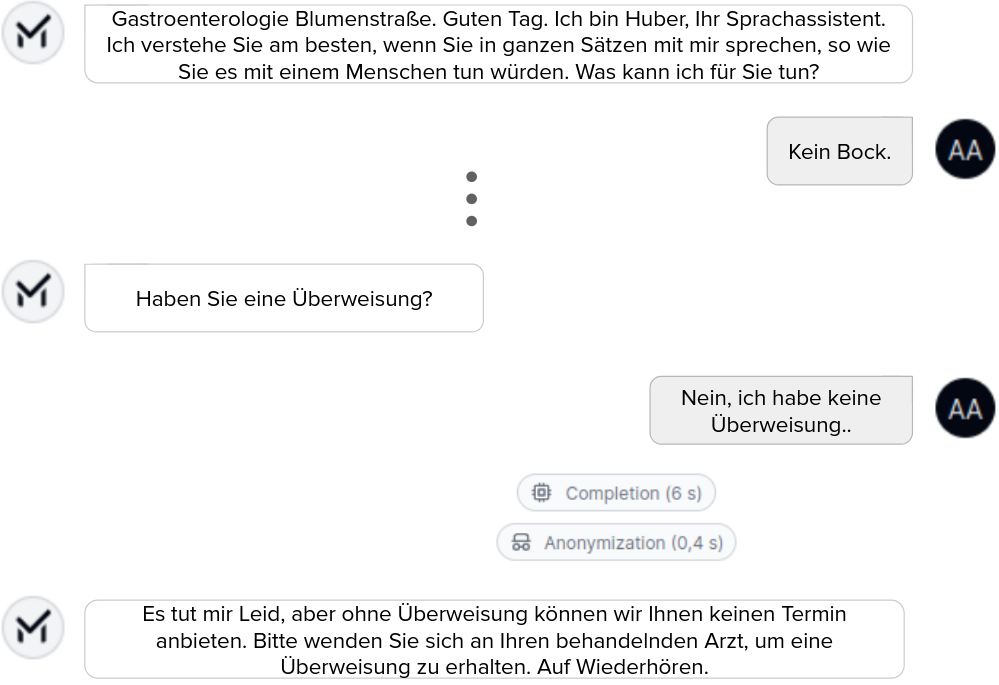
\includegraphics[width=0.26\textwidth]{figures/Dialog_UnhappyPath}}
\caption{Patient dialogues from happy paths (left) and unhappy paths (right)}
\label{fig:dialogues}
\end{center}
\end{figure}

The following subsections describe how the startup Mediform tackles the three challenges listed in the introduction. 

\subsection{Merge best practices}

To develop and fine-tune the MediVoice LLM, Mediform needs to merge best practices from three fields:
\begin{compactitem}
\item Data Science and Data Engineering, covering thousands of medical practice dialogues: anonymized dialogues from patients, non-AI generated dialogues, AI generated dialogues
\item Machine Learning, covering prompt engineering, pre-training and fine-tuning LLMs, and retrieval and agentic behavior
\item Agile development, to cope with new applications into uncharted realm, as described in the next subsection.
\end{compactitem}

\subsection{Validate product and LLM characteristics}

Since stakeholders (medics, medical assistants, health centers, call-centers, patients) don’t yet know what they want from the disruptive MediVoice application, their expectations evolve quickly and Mediform needs to be able to quickly update their requirements and targets correspondingly.Thus Mediform needs short iteration cycles with frequent feedback from the stakeholders. 

For instance, through short feedback cycles, Mediform soon revealed interesting findings on how patients behave on the phone:
\begin{compactitem}
\item due to previous bad experiences with extremely weak phone bots with horrible UX, patients are often very skeptical about MediVoice’s capabilities, or quickly become angry or impatient  (see Fig. 1 b). 
\item the unexpected patient behavior that 80+ year olds interact more effectively with MediVoice compared to younger patients [Mediform24].
\end{compactitem}

\subsection{Verify and evaluate LLMs}

Verifying and evaluating LLMs becomes a challenge for Mediform due to:
\begin{compactitem}
\item Using standard metrics and verification tools [Chang24] is too generic since we need to verify our LLMs in a business-centric way, to be able to evaluate that the model behaves correctly with regard to the desired characteristics and features. This means we need the right test driver (e.g. to enable individual business processes for each medical practice), and the right oracles (e.g. depending on the individual business process) and business-centric metrics (e.g. for defining correctness or priorities).
\item The LLMs capabilities with respect to NLU and reasoning is hard to evaluate because multiple semantically, but not syntactically close answers can be correct. For instance, we need to determine whether the LLM can cope with broken language, different languages, and speech-to-text errors? Furthermore, the model needs to understand practice specific business processes specified in natural language. The model needs to be able to generalize sufficiently and handle domain-specific corner cases.
\item The LLM is a black box and nondeterministic. Since the model is black box (except for some models offering top-k log-probabilities [Vaswani17]), so we can only measure via input-output pairs, and need to handle variations in the output for a fixed input, for instance with the help of semantic similarity and statistical testing.
\end{compactitem}

\section{The Solution at Mediform}

Having seen specific instances of the three challenges on the use-case MediVoice in the last section, this section shows Mediform’s solutions to each challenge.

\subsection{Merge best practices}

Most processes in the realm of data science and machine learning are an extension of CRISP-DM [CRISP99], the Cross-Industry Standard Process - Data Mining. For instance, [Farago23] is an extension that only focuses on prompt engineering, while CRISP-ML [Studer21] focuses on automotive and on waterfall processes, ignoring agility, which is necessary for short iterations with customer feedback for business-centric validation, and modern software development best practices. To the best of our knowledge, there is only one process and framework to enable both a data-centric yet business-centric and agile approach that is modern, AI-specific, and vendor-neutral: the Cognitive Process Management for AI (CPMAI) from Cognilytica, see Fig. \ref{fig:cpmai}. It has data at its core, which is read, extended or modified in each of the six phases:
\begin{compactitem}
\item {\bfseries Business Understanding}, which gathers an understanding of the business or organizational requirements and maps them to an AI solution
\item {\bfseries Data Understanding}, which identifies data (quality) requirements and data sources to address the problem
\item {\bfseries Data Preparation}, which prepares the training and test datasets by data cleansing, data aggregation, data augmentation, data labeling, and data transformation
\item {\bfseries Data Modeling}, which produces an AI solution, focusing on developing the ML model by choosing the model architecture, training technique, and hyperparameters, and by model training and optimization
\item {\bfseries Model Evaluation}, to check whether the AI solution meets the goals of the iteration, which are derived by the business or organizational requirements, by analyzing the confusion matrix and errors, by measuring metrics like precision and accuracy and more business-centric KPIs with respect to quality, performance and other ilities.
\item {\bfseries Model Operationalization}, to deploy the iteration’s AI solution to the stakeholders, performing model versioning, model deployment, model monitoring, and model staging.
\end{compactitem}

CPMAI embeds specific details and up-to-date data science and AI best practices, e.g.
\begin{compactitem}
\item which of the common seven patterns of AI [Cognilytica] are applied in the current AI solution, namely recognition, conversation \& human interaction, predictive analytics \& decisions, goal-driven systems, autonomous systems, patterns \& anomalies, hyper-personalization
\item how to train and optimize ML models
\item data science, big data, and visualization best practices.
\end{compactitem}

In contrast to CRISP-DM [CRISP99], CRISP-ML [Studer21] and other extensions, CPMAI does not merely offer a step from the Model Evaluation phase back to the Business Understanding phase, but has fully adopted modern agile practices: 
\begin{compactitem}
\item it incorporates Model Operationalization with modern DevOps practices, including staging
\item it integrates continuous customer feedback, enabled through staging
\item it offers high flexibility by allowing to switch between the six phases, bound together by data-centricity.
\end{compactitem}

\begin{figure}[hbt!]
  \begin{center}
  \vspace{-4mm}
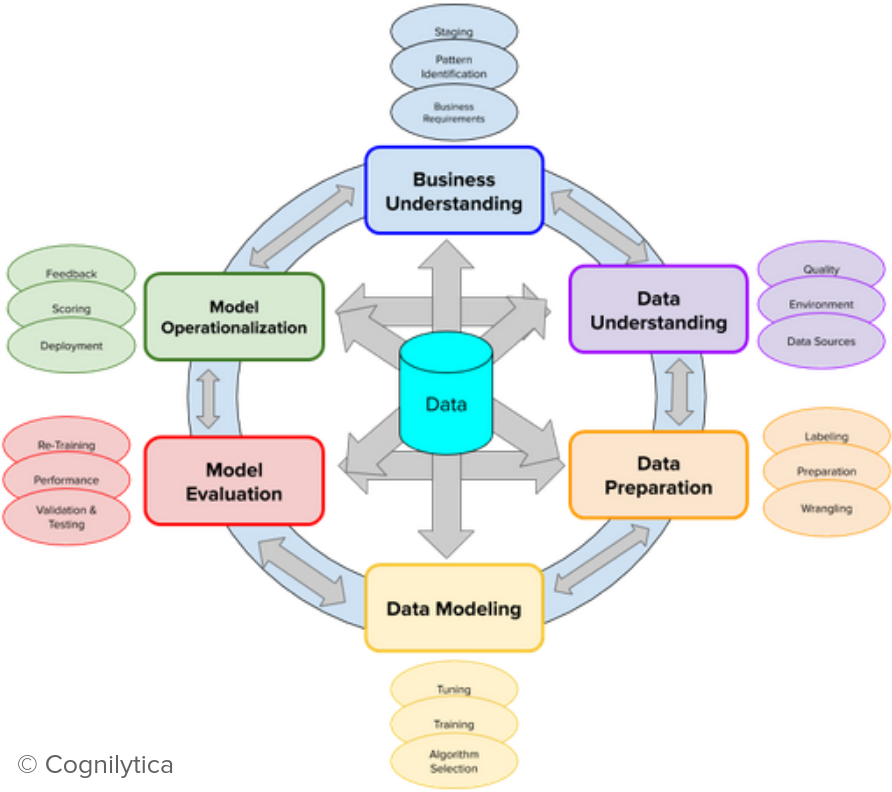
\includegraphics[width=0.4\textwidth]{figures/cpmai}
  \vspace{-4mm}
\caption{Cognilytica’s CPMAI process and framework}
\label{fig:cpmai}
\end{center}
\end{figure}

This flexibility and adoption of modern agile practices allows an easy embedding of up-to-date development best-practices, for instance Test-Driven Development (TDD). TDD is a test-first software development methodology, i.e. tests are written before the actual software is developed. In TDD, a red-green-refactor cycle is followed: a newly written test first fails, which motivates updating the system under test (SUT), but just with enough development to make the new test pass. The new and all old tests offer a safety-net to enable refactoring of both the tests and the SUT. Finally, we can iterate through the next loop of the red-green-refactor cycle.

CPMAI can easily be adapted to embed TDD:
\begin{compactitem}
\item The Data Preparation phase is the test-first phase, where a failing test is written
\item The Data Modeling phase is the development phase where the SUT is updated
\item The Model Evaluation phase is the subsequent test execution. If a test fails or we want to refactor the SUT, we move back to the Data Modeling phase. If we want to add another test or refactor tests, we move back to the Data Preparation phase.
\end{compactitem}

\subsection{Validate product and LLM characteristics}

CPMAI’s loop from Model Operationalization back to Business Understanding and Data Understanding allows frequent feedback from the stakeholders. For MediVoice, Mediform developed a backend for Interaction Analytics on anonymized patient dialogs. The evaluation (see Fig. \ref{fig:interactionanalytics}) helps in Business Understanding to find failing or not satisfying dialogs. In Data Understanding, an error analysis can be performed, to understand and prioritize use-cases and dialogs with regard to business requirements and business processes. The results of the error analysis help in the Data Preparation phase to update and extend the training and test sets by formulating dialogs that focus on the high priority business requirements and business processes. Thus, all data used within Mediform’s CPMAI instance are normalized to be dialogs with some metadata. The resulting dialogues or dialogue templates are based on the desired conversational behavior. The training and test sets cover a wide range of inputs and expected outputs, and are crucial for evaluating the LLM’s performance.

\begin{figure}[hbt!]
  \begin{center}
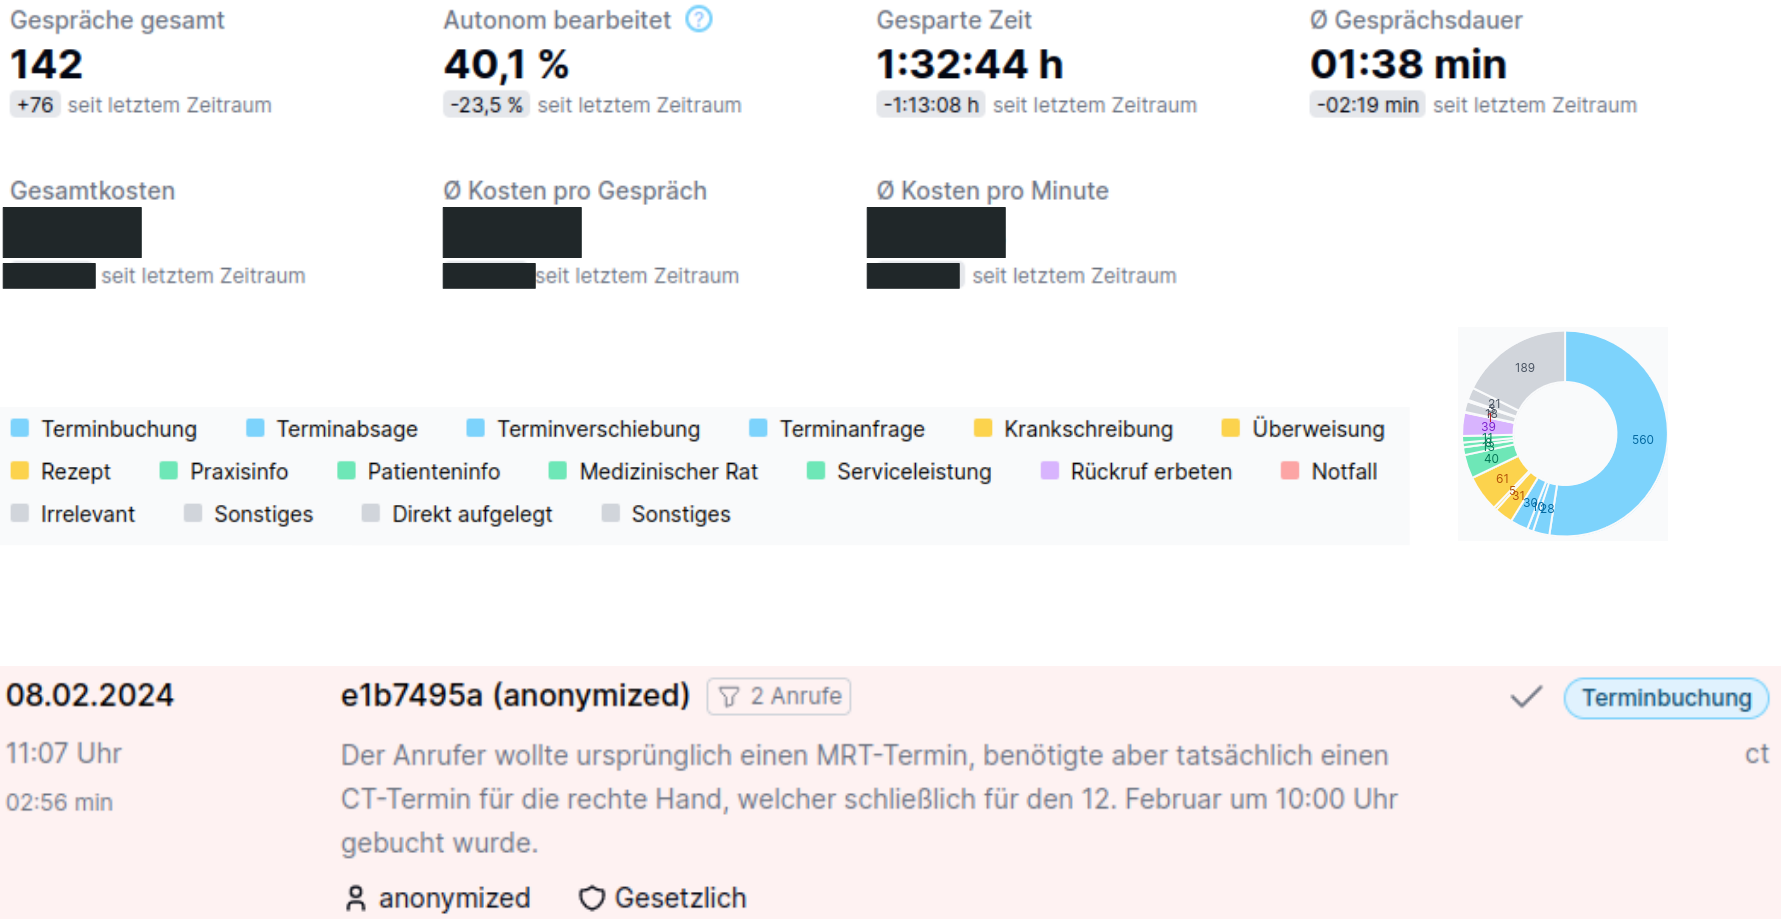
\includegraphics[width=0.5\textwidth]{figures/InteractionAnalytics}
  \vspace{-8mm}
\caption{Mediform’s Interaction Analytics on anonymized patient dialogues}
\label{fig:interactionanalytics}
\end{center}
\end{figure}

We extend CPMAI by an ATDD style LLM development: through the above process, the dialogues or dialogue templates within the test set are data-centric and can be considered as acceptance tests (ATs), i.e. as tests that are written based on the user’s requirements, i.e. in a customer-centric way. Thus ATs define the criteria for the software to be accepted, ensuring that the final product meets the user's needs. By using a TDD-like process (see previous section) within our CPMAI iterations, we extend CPMAI by an ATDD style LLM development, leading to \ATDLLMD{}. As opposed to classical ATDD, \ATDLLMD{} does not require all ATs to pass for overall acceptance of the LLM into production, rather a threshold for a metric like accuracy must be exceeded, as is usual for ML evaluations. When users know that the LLM has been fine-tuned and tested against customer-centric test cases with a suitable metric, their trust in the system also increases.


\subsection{Verify and evaluate LLMs}

To tackle the challenges of verifying and evaluating LLMs (see previous chapter), we develop our own novel testing tool {\bfseries LM-Eval}, enhancing EleutherAI’s Language Model Evaluation Harness [Gao23]. EleutherAI’s tool is known mainly from backing [HF24]. It contains many benchmarks, prompts, and metrics out of the box, but also offers the possibilities to extend them and evaluate custom models, making it very flexible.

For LM-Eval (see Fig. 4), we added, amongst others:
\begin{compactitem}
\item our own test driver to enable test execution of natural dialogues specified in our own format. For instance, our test set dialogues may contain template variables, their metadata may contain fields for business processes individual for the considered medical practice.
\item our own business-centric test oracles and metrics to evaluate natural dialogues, also with respect to NLU. For instance, we aggregate statistically, weighting individual results based on their semantic and business relevance.
\item features to perform non-deterministic black-box-testing. For instance, we do semantic comparisons (e.g. stricter for pre calls than msg calls, see Fig. \ref{fig:lmeval}) and allow specifying multiple alternative outputs.
\end{compactitem}

With our templated dialogue test sets as custom benchmarks, LM-Eval can evaluate our MediVoice models and cope with the challenges described in the previous chapter.

\begin{figure}[hbt!]
  \begin{center}
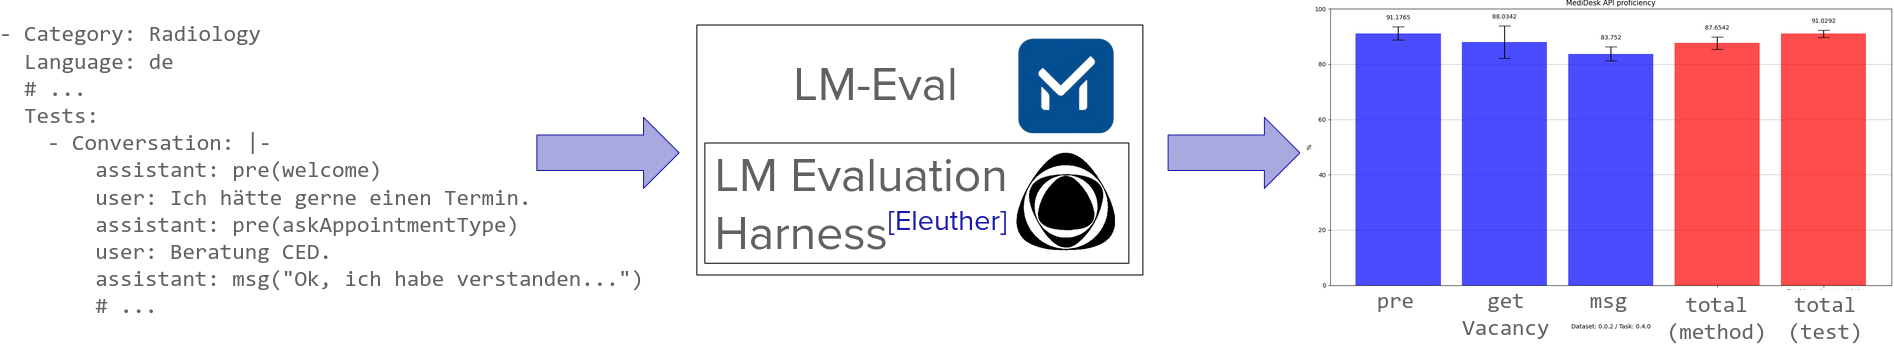
\includegraphics[width=0.5\textwidth]{figures/LMEval2}
  \vspace{-8mm}
\caption{Mediform’s LMEval Testing Framework}
\label{fig:lmeval}
\end{center}
\end{figure}

\subsection{Combining All Solutions}

With CPMAI and LM-Eval in place, we can perform a CPMAI roundtrip with \ATDLLMD{}: we iteratively collect dialogues from real patients in the Model Operationalization phase, i.e. the patients’ interactions with our novel phone bot. We anonymize them in a GDPR-conform way and then perform Business and Data Understanding on them with the help of our Interaction Analytics dashboard as well as manual exploration. Using the collected dialogues, especially those with undesired behavior, and insights from them, we create new dialogues with the corresponding desired behavior in the Data Preparation phase, specified as training data or acceptance tests that drive the current CPMAI iteration from red (failing acceptance tests) during Data Preparation, over Data Modeling (training), to green (passing acceptance tests) during Model Evaluation and Operationalization. Test execution and evaluation is performed by LM-Eval. As opposed to classical ATDD, not all acceptance tests need to become green, only enough to achieve the demanded metric, e.g. 85\% accuracy. This {\bfseries red-train-green cycle} in \ATDLLMD{} resembles ATDD, but integrates data science best practices. It also resembles CPMAI, but integrates modern software development and testing best practices.


\section{Conclusion}

In conclusion, applying ATDD to fine-tuning LLMs represents a significant step forward in developing more reliable, accurate, and user-centric AI language systems. This \ATDLLMD{} approach not only enhances the quality of outputs but also builds user confidence in AI technologies.

As future work, we are exploring ways to automate parts of this process, using AI itself to generate and update test scenarios. Furthermore, we are trying to directly incorporate feedback from various users to improve our model (as opposed to deriving feedback ourselves, and using the feedback to manually derive new test and training data).


\section{Acknowledgments}

Thanks go to Jochen Krause, CEO of Mediform GmbH, for offering the opportunity to work on this interesting task, and to my colleagues for the great work environment.

Thanks go to Cognilytica, LLC, which have the copyright and trademark for the CPMAI methodology and images (use here provided with written permission).


\section{Bibliography}

\hspace{3ex}[Akiba24] Akiba, Takuya, et al. "Evolutionary optimization of model merging recipes." arXiv preprint arXiv:2403.13187. 2024.

[Brown20] Brown, Tom, et al. "Language models are few-shot learners." Advances in neural information processing systems 33. 2020.

[Chang24] Chang, Yupeng, et al. "A survey on evaluation of large language models." ACM Transactions on Intelligent Systems and Technology 15.3 (2024): 1-45.

[Cognilytica] Cognilytica. “The Seven Patterns of AI”. https://www.cognilytica.com/the-seven-patterns-of-ai/

[CPMAI] Cognilytica: “Cognitive Cognitive Project Management For AI”, https://www.cognilytica.com/what-is-the-cognitive-project-management-for-ai-cpmai-methodology/

[CRISP99] “Cross Industry Standard Process for Data Mining 1.0”. https://web.archive.org/web/20220401041957/https:
//www.the-modeling-agency.com/crisp-dm.pdf

[Dettmers22] T. Dettmers, M. Lewis, Y. Belkada, and L. Zettlemoyer. LLM.int8(): 8-bit matrix multiplication for transformers at scale. Advances in Neural Information Processing Systems 35: Annual Conference on Neural Information Processing Systems 2022. 2022.

[Farago23] Faragó, David. "Engineering A Reliable Prompt For Generating Unit Tests-Prompt engineering for QA \& QA for prompt engineering." Softwaretechnik-Trends (STT). 2023.

[Gao23] Gao, Leo, et al. “A framework for few-shot language model evaluation. 2023. https://zenodo.org/records/10256836

[Github23] Github. “How to build an enterprise LLM application: Lessons from GitHub Copilot”. https://github.blog/2023-09-06-how-to-build-an-enterprise-llm-application-lessons-from-github-copilot/.

[Gra23] Gramener Blog: "Large Language Models (LLMs): A Technology Gifted by Aliens Without a Manual ". 2023. https://blog.gramener.com/large-language-models-llms-technology

[HF24] Hugging Face. "Open LLM Leader- board". 2024. https://huggingface.co/spaces/
HuggingFaceH4/open$\_$llm$\_$leaderboard

[Hosseini20] Hosseini-Asl, Ehsan, et al. "A simple language model for task-oriented dialogue." Advances in Neural Information Processing Systems 33. 2020.

[Kaplan20] Kaplan, Jared, et al. "Scaling laws for neural language models." arXiv preprint arXiv:2001.08361. 2020. 

[Ke23] Ke, Zixuan, et al. "Continual pre-training of language models." arXiv preprint arXiv:2302.03241. 2023.

[Liu22] Liu, Haokun, et al. "Few-shot parameter-efficient fine-tuning is better and cheaper than in-context learning." Advances in Neural Information Processing Systems 35. 2022.

[Mediform24] Mediform: “Ältere Menschen buchen problemlos Termine via MediVoice”. https://tinyurl.com/medivoice.

[MediVoice] Mediform. “Die Revolution für das Praxistelefon”. https://mediform.io/medivoice/

[Minaee24] Minaee, Shervin, et al. "Large language models: A survey." arXiv preprint arXiv:2402.06196. 2024.

[Röttger24] Röttger, Nils, Gerhard Runze, and Verena Dietrich. Basiswissen KI-Testen: Qualität von und mit KI-basierten Systemen: Aus-und Weiterbildung zum Certified Tester AI Testing: Foundation Level Specialist nach ISTQB®-Standard. Dpunkt. verlag, 2024.

[Studer21] Studer, Stefan, et al. "Towards CRISP-ML (Q): a machine learning process model with quality assurance methodology." Machine learning and knowledge extraction 3.2. 2021.

[Vaswani17] Vaswani, Ashish, et al. "Attention is all you need." Advances in neural information processing systems 30. 2017.

[Wang24] Chen, Wang, et al. "Systems engineering issues for industry applications of large language model." Applied Soft Computing 151. 2024.

\iffalse

\bibliographystyle{unsrt}
\begin{thebibliography}{10}
\footnotesize
\bibitem{AlSabbagh22} Al-Sabbagh, Khaled Walid et al. {\em Improving test case selection by handling class and attribute noise.} Journal of Systems and Software 183. 2022.
\bibitem{Baviskar21} Baviskar, Dipali et al. {\em Multi-Layout Unstructured Invoice Documents Dataset: A Dataset for Template-Free Invoice Processing and Its Evaluation Using AI Approaches.}. IEEE Access, vol. 9. 2021.
\bibitem{Breck19} Breck, Eric, et al. {\em Data Validation for Machine Learning.} MLSys. 2019.
\bibitem{Brodley96} Brodley, Carla, and Friedl, Mark. {\em Identifying and eliminating mislabeled training instances.} Proceedings of the National Conference on Artificial Intelligence. 1996.
\bibitem{Budach22} Budach, Lukas, et al. {\em The Effects of Data Quality on Machine Learning Performance.} arXiv preprint. 2022.
\bibitem{Cohen60} Cohen, Jacob. {\em A coefficient of agreement for nominal scales.} EPM. 1960.
\bibitem{DAI} Datacentric AI Resource Hub: https://datacentricai.org. 
\bibitem{DMT} https://huggingface.co/blog/data-measurements-tool. 
\bibitem{Felderer19} Foidl, Harald, and Michael Felderer. {\em Risk-based data validation in machine learning-based software systems.} Proceedings of the 3rd ACM SIGSOFT. 2019.
\bibitem{GE} Great Expectations Blog Post. {\em You Are What You Eat: Why Data Quality Matters for Machine Learning.} https://greatexpectations.io/blog/why-data-quality-matters-for-machine-learning. 
\bibitem{InvoiceLG} {\em Concise Invoice Labeling Guide}. http://tinyurl.com/InvoiceLabelingGuide. 
\bibitem{Neves21} Mariana Neves, Jurica Seva. {\em An extensive review of tools for manual annotation of documents.} Briefings in Bioinformatics, Volume 22, Issue 1, January 2021, Pages 146–163, https://doi.org/10.1093/bib/bbz130. 2021
\bibitem{Northcutt21} Northcutt, Curtis, Lu Jiang, and Isaac Chuang. {\em Confident learning: Estimating uncertainty in dataset labels.} Journal of Artificial Intelligence Research 70. 2021.
\bibitem{Paullada20} Paullada, Amandalynne, et al. {\em Data and its (dis) contents: A survey of dataset development and use in machine learning research.} Patterns 2.11. 2021.
\bibitem{CLIP} Radford, Alec, et al. {\em Learning transferable visual models from natural language supervision.} International Conference on Machine Learning. PMLR. 2021.
\bibitem{Sambasivan21} Sambasivan, Nithya, et al. {\em ``Everyone wants to do the model work, not the data work'': Data Cascades in High-Stakes AI.} Proceedings of the CHI Conference on Human Factors in Computing Systems. 2021.
\bibitem{Batini06} Scannapieco, Monica. {\em Data Quality: Concepts, Methodologies and Techniques. Data-Centric Systems and Applications.} Springer. 2006.
\bibitem{Scheuerman21} Scheuerman, Morgan Klaus et al. {\em Do datasets have politics? Disciplinary values in computer vision dataset development.} Proceedings of the ACM on HCI. 2021.
\bibitem{Sluban10} Sluban, Borut, Gamberger, Dragan, and Lavra, Nada. {\em Advances in class noise detection.} ECAI. 2010.
\bibitem{Tagliabue21} Tagliabue, Jacopo. {\em You do not need a bigger boat: recommendations at reasonable scale in a (mostly) serverless and open stack.} Fifteenth ACM Conference on Recommender Systems. 2021.
\bibitem{Tseng20} Tseng, Tina, Amanda Stent, and Domenic Maida. {\em Best Practices for Managing Data Annotation Projects.} arXiv preprint arXiv:2009.11654. 2020.

\bibitem{Barrett19} Barrett, Leslie, and Michael W. Sherman. {\em Improving ML Training Data with Gold-Standard Quality Metrics}. 2019.
  
\end{thebibliography}
\fi
\end{document}
